\chapter{Covering Projections}

A few chapters ago we talked about what a fundamental group was,
but we didn't actually show how to compute any of them
except for the most trivial case of a simply connected space.
In this chapter we'll introduce the notion of a \emph{covering projection}.

\section{Even Coverings and Covering Projections}
\prototype{$\RR$ covers $S^1$.}
What we want now is a notion where a big space $E$, a ``covering space'',
can be projected down onto a base space $B$ in a nice way.
Here is the notion of ``nice'':
\begin{definition}
	Let $p : E \to B$ be a continuous function.
	Let $U$ be an open set of $B$.
	We call $U$ \vocab{evenly covered} (by $p$) if $p\pre(U)$ is a disjoint union of open sets (possibly infinite) such that $p$ restricted to any of these sets is a homeomorphism.  
\end{definition}
Picture:
\begin{center}
	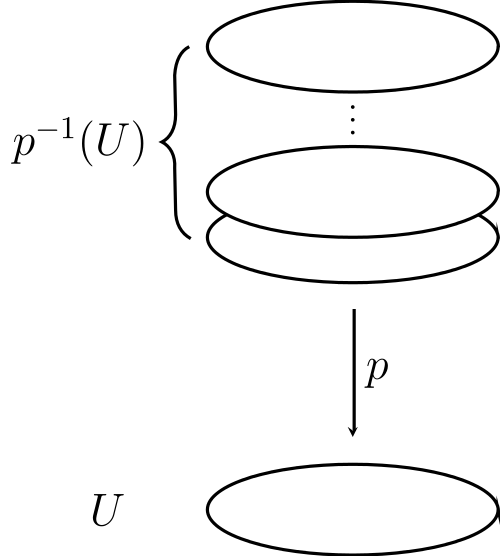
\includegraphics[width=4cm]{media/even-covering.png}
	% COPYRIGHT ISSUE
\end{center}
All we're saying is that $U$ is evenly covered if its pre-image
is a bunch of copies of it. (Actually, a little more: each of the pancakes is homeomorphic to $U$, but we also require that $p$ is the homeomorphism.)

\begin{definition}
	A \vocab{covering projection} $p : E \to B$
	is a continuous map such that every base point $b \in B$
	has a neighborhood $U \ni b$ which is evenly covered by $p$.
\end{definition}
\begin{ques}
	Why must a covering projection be surjective?
\end{ques}

Here is the most stupid example of a covering projection.
\begin{example}[Tautological Covering Projection]
	Let's take $n$ disconnected copies of any space $B$:
	formally, $E = B \times \{1, \dots, n\}$ with the discrete topology
	on $\{1, \dots, n\}$.
	Then there exists a tautological covering projection
	$E \to B$ by $(x,m) \mapsto x$;
	we just project all $n$ copies.

	This is a covering projection because \emph{every} open set in $B$
	is evenly covered.
\end{example}
This is not really that interesting because $B \times [n]$ is not path-connected.

A much more interesting example is that of $\RR$ and $S^1$.

\begin{example}[Covering Projection of $S^1$]
	Take $p : \RR \to S^1$ by $\theta \mapsto e^{2\pi i \theta}$.  This is essentially wrapping the real line into a single helix and projecting it down.
\end{example}
\missingfigure{helix}

We claim this is a covering projection.
Indeed, consider the point $1 \in S^1$ (where we view $S^1$ as the unit circle in the complex plane). We can draw a small neighborhood of it
whose pre-image is a bunch of copies in $\RR$.
\begin{center}
	\begin{asy}
		size(12cm);

		real[] t = {-2,-1,0,1,2};
		xaxis(-3.5,3.5, graph.LeftTicks(Ticks=t), Arrows); 

		pen bloo = blue+1.5;

		dotfactor *= 2;
		pair A,B;
		for (real x = -2; x <= 2; ++x) {
			A = (x-0.2, 0); B = (x+0.2, 0);
			draw(A--B, bloo); opendot(A, blue); opendot(B, blue);
		}
		MP("\mathbb R", (3,0), dir(90));

		add(shift( (0,3) ) * CC());

		path darrow = (0,2.5)--(0,1.5);
		MP("p", midpoint(darrow), dir(0));
		draw(darrow, EndArrow);

		real r = 1.4;
		draw(scale(r)*unitcircle);
		MP("S^1", r*dir(45), dir(45));
		A = r*dir(-20);
		B = r*dir(20);
		draw(arc(origin, A, B), bloo);
		opendot(A, blue); opendot(B, blue);
		dot("$1$", r*dir(0), dir(0));
	\end{asy}
\end{center}

Note that not all neighborhoods work this time: notably, $U = S^1$ does not work because the pre-image would be the entire $\RR$.

\begin{example}[Covering of $S^1$ by itself]
	The map $S^1 \to S^1$ by
	$z \mapsto z^{3}$ is also a covering projection.
	Can you see why?
\end{example}

\begin{example}
	[Covering Projections of $\CC \setminus \{0\}$]
	For those comfortable with complex arithmetic,
	\begin{enumerate}[(a)]
		\ii The exponential map $\exp : \CC \to \CC \setminus \{0\}$
		is a covering projection.
		\ii For each $n$, the $n$th power map
		$-^n: \CC \setminus \{0\} \to \CC \setminus \{0\}$
		is a covering projection.
	\end{enumerate}
\end{example}

\section{Lifting Theorem}
\prototype{$\RR$ covers $S^1$.}
Now here's the key idea: we are going to try to interpret paths in $B$ as loops in $\RR$.
This is often much simpler.
For example, we had no idea how to compute the fundamental group of $S^1$,
but the fundamental group of $\RR$ is just the trivial group.
So if we can interpret loops in $S^1$ as loops in $\RR$, that might (and indeed it does!) make computing $\pi_1(S^1)$ tractable.

\begin{definition}
	Let $\gamma : [0,1] \to B$ be a path and $p : E \to B$ a covering projection.
	A \vocab{lifting} of $\gamma$ is a path $\tilde\gamma : [0,1] \to E$
	such that $p \circ \tilde\gamma = \gamma$.
\end{definition}
Picture:
\begin{diagram}
	&&& E \\
	&& \ruTo(3,2)^{\tilde \gamma} & \dTo_p \\
	[0,1] & \rTo^{\gamma} && B
\end{diagram}

\begin{example}[Typical Example of Lifting]
	Take $p : \RR \to S^1 \subseteq \CC$ by $\theta \mapsto e^{2 \pi i \theta}$
	(so $S^1$ is considered again as the unit circle).
	Consider the path $\gamma$ in $S^1$ which starts at $1 \in \CC$
	and wraps around $S^1$ once, counterclockwise, ending at $1$ again.
	In symbols, $\gamma : [0,1] \to S^1$ by $t \mapsto e^{2\pi i t}$.

	Then one lifting $\tilde\gamma$ is the path which walks from $0$ to $1$.
	In fact, \emph{for any integer $n$}, walking from $n$ to $n+1$ works.

	\begin{center}
		\begin{asy}
			size(6cm);

			real[] t = {-1,0,1,2};
			xaxis(-2,3, graph.LeftTicks(Ticks=t), Arrows); 
			MP("\mathbb R", (2.5,0), dir(90));
			path gt = (0,0.3)--(1,0.3);
			draw(gt, blue, EndArrow);
			label("$\tilde\gamma$", midpoint(gt), dir(90), blue);
			add(shift( (0,3) ) * CC());

			path darrow = (0,2.5)--(0,1.5);
			MP("p", midpoint(darrow), dir(0));
			draw(darrow, EndArrow);

			real r = 1.2;
			draw(scale(r)*unitcircle);
			MP("S^1", r*dir(45), dir(45));
			dot("$1$", r*dir(0), dir(0));
			path g = dir(20)..dir(100)..dir(180)..dir(260)..dir(340);
			draw(g, red, EndArrow);
			label("$\gamma$", midpoint(g), -dir(midpoint(g)), red);

			MP("p(0) = 1", (2.5,0.5));
			MP("p(1) = 1", (2.5,0));
		\end{asy}
	\end{center}

	Similarly, the counterclockwise path from $1 \in S^1$ to $-1 \in S^1$
	has a lifting: for some integer $n$, the path from $n$ to $n+\half$.
	\label{example:lifting_circle}
\end{example}

The above is the primary example of a lifting.
It seems like we have the following structure: given a path $\gamma$
in $B$ starting at $b_0$, we start at any point in the fiber $p\pre(b_0)$.
(In our prototypical example, $B = S^1$, $b_0 = 1 \in \CC$
and that's why we start at any integer $n$.)
After that we just trace along the path in $B$, and we get
a corresponding path in $E$.
\begin{ques}
	Take a path $\gamma$ in $S^1$ with at $\gamma(0) = 1 \in \CC$.
	Convince yourself that once we select an integer $n \in \RR$,
	then there is exactly one lifting starting at $n$.
\end{ques}

It turns out this is true more generally.
\begin{theorem}[Lifting Paths]
	Suppose $\gamma : [0,1] \to B$ is a path with $\gamma(0) = \gamma(1) = b_0$, and 
	$ p : (E,e_0) \to (B,b_0) $
	is a covering projection.
	Then there exists a \emph{unique} lifting $\tilde\gamma : [0,1] \to E$
	such that $\tilde\gamma(0) = e_0$.
\end{theorem}
\begin{proof}
	For every point $b \in B$, consider an evenly covered neighborhood $U_b$ in $B$.
	Then the family of open sets
	\[ \left\{ \gamma\pre(U_b) \mid b \in B \right\} \]
	is an open cover of $[0,1]$.
	Since $[0,1]$ is a compact metric space, we can take a finite subcover.
	It follows that we can chop $[0,1]$ into finitely many disjoint closed intervals
	$[0,1] = I_1 \sqcup I_2 \sqcup \dots \sqcup I_N$ in that order,
	with the property that for every $I_k$, $\gamma``(I_k)$ is contained
	in some $U_b$.

	We'll construct $\tilde\gamma$ interval by interval now,
	starting at $I_1$.
	Initially, place a robot at $e_0 \in E$ and a mouse at $b_0 \in B$.
	For each interval $I_k$, the mouse moves around according
	to however $\gamma$ behaves on $I_k$.
	But the whole time it's in some evenly covered $U_k$; the fact that $p$ is a covering projection tells us that there's are several copies of $U_k$ living in $E$. Exactly one of them, say $V_k$, contains our robot.
	So the robot just mimics the mouse until it gets to the end of $I_k$.
	Then the mouse is in some new evenly covered $U_{k+1}$,
	and we can repeat.
\end{proof}

The theorem can be generalized to a diagram
\begin{diagram}
	&& (E, e_0) \\
	& \ruTo^{\tilde f} & \dTo_{p} \\
	(Y,y_0) & \rTo^{f} & (B, b_0)
\end{diagram}
where $Y$ is some general path-connected space, as follows.
\begin{theorem}[General Lifting Criterion]
	Let $f: (Y,y_0) \to (B, b_0)$ be continuous and consider a covering projection $p : (E, e_0) \to (B, b_0)$.
	(As usual, $Y$, $B$, $E$ are path-connected.)
	Then a lifting  $\tilde f$ with $\tilde f(y_0) = e_0$ if and only if
	\[ f_\ast``(\pi_1(Y, y_0)) \subseteq p_\ast``(\pi_1(E, e_0)). \]
	(Here we view both sides as subgroups of $\pi_1(B, b_0)$.)
	If this lifting exists, it is unique.
\end{theorem}
As $p$ is injective, we actually have $p_\ast``(\pi_1(E, e_0)) \cong \pi_1(E, e_0)$.
But in this case we are interested in the actual elements, not just the isomorphism classes of the groups.
\begin{ques}
	What happens if we put $Y= [0,1]$?
\end{ques}

\begin{remark}[Lifting Homotopies]
	Here's another cool special case:
	Recall that a homotopy can be encoded as a continuous function $[0,1] \times [0,1] \to X$.
	But $[0,1] \times [0,1]$ is also simply connected.
	Hence given a homotopy $\gamma_1 \simeq \gamma_2$ in the base space $B$, we can lift it to get
 a homotopy $\tilde\gamma_1 \simeq \tilde\gamma_2$ in $E$.
\end{remark}

\section{Lifting Correspondence}
\prototype{$(\RR,0)$ covers $(S^1,1)$.}
Let's return to the task of computing fundamental groups.
Consider a covering projection $p : (E, e_0) \to (B, b_0)$.

A loop $\gamma$ can be lifted uniquely to $\tilde\gamma$ in $E$
which starts at $e_0$ and ends at some point $e$ in the fiber $p\pre(b_0)$.
You can easily check that this $e \in E$ does not change if we
pick a different path $\gamma'$ homotopic to $E$.
\begin{ques}
	Look at the picture in \Cref{example:lifting_circle}.

	Put one finger at $1 \in S^1$, and one finger on $0 \in \RR$.
	Trace a loop homotopic to $\gamma$ in $S^1$ (meaning, you can
	go backwards and forwards but you must end with exactly one full
	counterclockwise rotation)
	and follow along with the other finger in $\RR$.

	Convince yourself that you have to end at the point $1 \in \RR$.
\end{ques}

Thus every homotopy class of a loop at $b_0$ (i.e.\ an element of $\pi_1(B, b_0)$) can be associated with some $e$ in the fiber of $b_0$.
The below proposition summarizes this and more.
\begin{proposition}
	Let $p : (E,e_0) \to (B,b_0)$ be a covering projection.
	Then we have a function of sets
	\[ \Phi : \pi_1(B, b_0) \to p\pre(b_0) \]
	by $[\gamma] \mapsto \tilde\gamma(1)$, where $\tilde\gamma$
	is the unique lifting starting at $e_0$.
	Furthermore,
	\begin{itemize}
		\ii If $E$ is path-connected, then $\Phi$ is surjective.
		\ii If $E$ is simply connected, then $\Phi$ is injective.
	\end{itemize}
\end{proposition}
\begin{ques}
	Prove that $E$ path-connected implies $\Phi$ is surjective.
	(This is really offensively easy.)
\end{ques}
\begin{proof}
	To prove the proposition, we've done everything except show
	that $E$ simply connected implies $\Phi$ injective.
	To do this suppose that $\gamma_1$ and $\gamma_2$ are loops
	such that $\Phi([\gamma_1]) = \Phi([\gamma_2])$.

	Applying lifting, we get paths $\tilde\gamma_1$ and $\tilde\gamma_2$
	both starting at some point $e_0 \in E$ and ending at some point $e_1 \in E$.
	Since $E$ is simply connected that means they are \emph{homotopic},
	and we can write a homotopy $F : [0,1] \times [0,1] \to E$
	which unites them.
	But then consider the composition of maps
	\[ [0,1] \times [0,1] \taking{F} E \taking{p} B. \]
	You can check this is a homotopy from $\gamma_1$ to $\gamma_2$.
	Hence $[\gamma_1] \simeq [\gamma_2]$, done.
\end{proof}

This motivates the following definition.
\begin{definition}
	A \vocab{universal cover} of a space $B$ is a covering projection
	$p : E \to B$ where $E$ is simply connected (and in particular path-connected).
\end{definition}
\begin{abuse}
	When $p$ is understood, we sometimes just say $E$ is the universal cover.
\end{abuse}

\begin{example}[Fundamental Group of $S^1$]
	Let's return to our standard $p : \RR \to S^1$.
	Since $\RR$ is is simply connected, this is a universal cover of $S^1$.
	And indeed, the fiber of any point in $S^1$
	is a copy of the integers: naturally in bijection with loops in $S^1$.
	
	You can show (and it's intuitively obvious) that the bijection
	\[ \Phi : \pi_1(S^1) \leftrightarrow \ZZ \]
	is in fact a group homomorphism if we equip $\ZZ$ with its
	additive group structure $\ZZ_+$.
	Since it's a bijection, this leads us to conclude $\pi_1(S^1) \cong \ZZ$.
\end{example}

\section{Regular Coverings}
I want to talk a little about a special type of covering now: those
that arise from group actions.

Let $X$ be a topological space and $G$ a group acting on its points.
Thus for every $g$, we get a map $X \to X$ by 
\[ x \mapsto g \cdot x. \]
We require that this map is continuous for every $g \in G$.\footnote{%
	Another way of phrasing this as saying that the action,
	interpreted as a map $X \times G \to X$, should be continuous,
	where $G$ on the left-hand side is interpreted as a set with
	the discrete topology.}

Then we can consider a topological space $X/G$ defined by fusing any points
in the same orbit of this action.
(The open sets of $X/G$ are just the open sets of $X$ after this identification.)
In other words, the points of $X/G$ are the orbits of the action.
Then we get a natural ``projection''
\[ X \to G/X \]
by simply sending every points to the orbit it lives in.
\begin{definition}
	Such a projection is called \vocab{regular}.
	(Terrible, I know.)
\end{definition}

\begin{example}[$\RR \to S^1$ is regular]
	Let $G = \ZZ_+$, $X = \RR$
	and define the group action of $G$ on $X$ by 
	\[ n \cdot x = n + x \]
	You can then think of $X/G$ as ``real numbers modulo $1$'',
	with $[0,1)$ a complete set of representatives and $0 \sim 1$.
	\begin{center}
		\begin{asy}
			size(9cm);
			dotfactor *= 2;
			pair A = MP("0", (-5.1,0), 1.4*dir(90));
			pair B = MP("1", (-3,0), 1.4*dir(90));
			draw(A--B);
			D("\frac13", (-4.4,0), 1.4*dir(90));
			D("\frac23", (-3.7,0), 1.4*dir(90));
			MP("\mathbb R / G", (-4,-0.6), dir(-90));
			dot(A); opendot(B);
			draw(unitcircle);
			draw( (-2.4,0)--(-1.6,0), EndArrow);
			dot("$0=1$", dir(0), dir(0));
			dot("$\frac13$", dir(120), dir(120));
			dot("$\frac23$", dir(240), dir(240));
			label("$S^1$", origin, origin);
		\end{asy}
	\end{center}
	So we can identify $X/G$ with $S^1$
	and the associated regular projection
	is just our usual $\exp : \theta \mapsto e^{2i\pi \theta}$.
\end{example}
	
\begin{example}[The Torus]
	Let $G = \ZZ_+ \times \ZZ_+$ and $X = \RR^2$,
	and define the group action of $G$ on $X$ by $(m,n) \cdot (x,y)
	= (m+x, n+y)$.
	Again, since $[0,1)^2$ is a complete set of representatives,
	you can think of it as a unit square with the edges identified.

	This is a torus, also known as $S^1 \times S^1$,
	and it gives us a covering projection $\RR^2 \to S^1 \times S^1$.
\end{example}

\begin{example}[$\mathbb {RP}^2$]
	Let $G = \Zc 2 = \left<T \mid T^2 = 1\right>$ and
	let $X = S^2$ be the surface of the sphere,
	viewed as a subset of $\RR^3$.
	We'll let $G$ act on $X$ by sending $T \cdot \vec x = - \vec x$;
	hence the orbits are pairs of opposite points (e.g.\ North and South pole).

	Let's draw a picture of a space.
	All the orbits have size two:
	every point below the equator gets fused with a point above the equator.
	As for the points on the equator, we can take half of them; the other half
	gets fused with the corresponding antipodes.

	Now if we flatten everything, you can think of the result as disk
	with half its boundary.
	The resulting space has a name: \emph{real projective $2$-space},
	denote $\mathbb{RP}^2$.
	\begin{center}
		\begin{asy}
			size(3cm);
			dotfactor *= 2;
			draw(dir(-90)..dir(0)..dir(90));
			draw(dir(90)..dir(180)..dir(-90), dashed);
			fill(unitcircle, rgb(0.9,0.9,0.9));
			dot(dir(90));
			opendot(dir(-90));
			label("$\mathbb{RP}^2$", origin, origin);
		\end{asy}
	\end{center}

	It should be familiar to those of you who do projective geometry.
	The points in the ``interior'' are your usual Eucliean points,
	and the points in the equator are the points at infinity
	(which explains why they get paired up like that).

	This gives us a covering projection $S^2 \to \mathbb{RP}^2$
	(note that the pre-image of a sufficiently small patch is just two copies
	of it on $S^2$.)
\end{example}
\begin{example}
	[Fundamental Group of $\mathbb{RP}^2$]
	As above, we saw that there was a covering projection
	$S^2 \to \mathbb{RP}^2$.
	Moreover the fiber of any point has size two.
	Since $S^2$ is simply connected, we have a natural bijection
	$\pi_1(\mathbb{RP}^2)$ to a set of size two; that is,
	\[ \left\lvert \pi_1(\mathbb{RP}^2) \right\rvert = 2. \]
	This can only occur if $\pi_1(\mathbb{RP}^2) \cong \Zc 2$,
	as there is only one group of order two!
\end{example}

\begin{ques}
	Show each of the continuous maps $x \mapsto g \cdot x$ is in fact a homeomorphism.
	(Name its continuous inverse).
\end{ques}
% WOW I thought this was always a covering projection gg

\section{The Algebra of Fundamental Groups}
\prototype{$S^1$, with fundamental group $\ZZ$.}
Next up, we're going to turn functions between spaces into homomorphisms of fundamental groups.

Let $X$ and $Y$ be topological spaces and $f : (X, x_0) \to (Y, y_0)$.
Recall that we defined a group homomorphism
\[ f_\sharp : \pi_1(X, x_0) \to \pi_1(Y_0, y_0) 
	\quad\text{by}\quad
	[\gamma] \mapsto [f \circ \gamma] \]
which gave us a functor $\catname{Top}_\ast \to \catname{Gp}$.

More importantly, we have the following result.
\begin{proposition}
	Let $p : (E,e_0) \to (B,b_0)$ be a covering projection of path-connected spaces.
	Then the homomorphism $p_\sharp : \pi_1(E, e_0) \to \pi_1(B, b_0)$ is \emph{injective}.
	Hence $p_\sharp ``(\pi_1(E, e_0))$ is an isomorphic copy of $\pi_1(E, e_0)$ 
	as a subgroup of $\pi_1(B, b_0)$.
\end{proposition}
\begin{proof}
	We'll show $\ker p_\sharp$ is trivial.
	It suffices to show if $\gamma$ is a nulhomotopic loop in $B$ 
	then its lift is nulhomotopic.

	By definition, there's a homotopy $F : [0,1] \times [0,1] \to B$
	taking $\gamma$ to the constant loop $1_B$.
	We can lift it to a homotopy $\tilde F : [0,1] \times [0,1] \to E$
	that establishes $\tilde\gamma \simeq \tilde 1_B$.
	But $1_E$ is a lift of $1_B$ (duh) and lifts are unique.
\end{proof}

\begin{example}[Subgroups of $\ZZ_+$]
	Let's look at the space $S^1$ with fundamental group $\ZZ_+$.
	The group $\ZZ_+$ has two types of subgroups:
	\begin{itemize}
		\ii The trivial subgroup.
		This corresponds to the canonical projection $\RR \to S^1$,
		since $\pi_1(\RR)$ is the trivial group ($\RR$ is simply connected)
		and hence its image in $\ZZ_+$ is the trivial group.
		\ii $n\ZZ$ for $n \ge 1$.
		This is given by the covering projection $S^1 \to S^1$
		by $z \mapsto z^n$.
		The image of a loop in the covering $S^1$ is a ``multiple of $n$''
		in the base $S^1$.
	\end{itemize}
\end{example}

It turns out that these are the \emph{only} covering projections of $S^n$ by path-connected spaces: there's one for each subgroup of $\ZZ_+$.
(We don't care about disconnected spaces because, again, a covering projection
via disconnected spaces is just a bunch of unrelated ``good'' coverings.)
For this statement to make sense I need to tell you what it means for
two covering projections to be equivalent.

This is done most naturally in the language of category theory.
Fix a space $B$.
We can build a category whose objects are covering projections $p : E \to B$.
Then given two covering projections $p_1 : E_1 \to B$ and $p_2 : E_2 \to B$
a \vocab{map of covering projections} is a continuous function $f : E_1 \to E_2$
such that $p_2 \circ f = p_1$.
\begin{diagram}
	E_1 & \rTo^f && E_2 \\
	& \rdTo(3,2)_{p_1} && \dTo_{p_2} \\
	&&& B
\end{diagram}
Then we can just use the categorical definition of isomorphism:
there exist two such maps which are inverses.

It's an absolute miracle that this is true more generally:
the greatest triumph of covering spaces is the following result.
Suppose a space $X$ has the following conditions.
\begin{definition}
	A space $X$ is called \vocab{locally connected} if for every point $x \in X$
	has a connected neighborhood $U$.
\end{definition}
\begin{definition}
	A space $X$ is \vocab{semi-locally simply connected} if for every point $x \in X$
	there is a neighborhood $U$ such that all loops in $U$ are nulhomotopic.
	(But the contraction need not take place in $U$.)
\end{definition}
\begin{example}[These Conditions Are Weak]
	Pretty much every space I've shown you has these two properties.
	In other words, they are rather mild conditions, and you can think of them as just
	saying ``the space is not too pathological''.
\end{example}
Then we get the following theorem.
\begin{theorem}[Group Theory via Covering Spaces]
	Suppose $B$ is a connected, locally connected, semi-locally simply connected space.
	Then:
	\begin{itemize}
		\ii Every subgroup of $H \subseteq \pi_1(B)$ corresponds
		to exactly one covering projection $p : E \to B$
		with $E$ path-connected (up to isomorphism).

		(Specifically, $H$ is the image of $\pi_1(E)$ in $\pi_1(B)$ through $p_\sharp$.)
		\ii Moreover, the \emph{normal} subgroups of $\pi_1(B)$
		correspond exactly to the regular covering projections.
	\end{itemize}
\end{theorem}
Hence it's possible to understand the group theory of $\pi_1(B)$ completely
in terms of the covering projections.

Moreover, this is how the ``universal cover'' gets its name:
it is the one corresponding to the trivial subgroup of $\pi_1(B)$.
Actually, you can show that it really is universal in the sense
that if $p : E \to B$ is another covering projection,
then $E$ is in turn covered by the universal space.
More generally, if $H_1 \subseteq H_2 \subseteq G$ are subgroups,
then the space corresponding to $H_2$ can be covered by the space
corresponding to $H_1$.

% According to \cite{ref:covering_all_we_know}, this statement and
% its extension to group actions are ``pretty much all there is to know
% about covering projections''.

\section\problemhead
\todo{find problems}
